\chapter{凸优化}\label{convex-optimization}
优化与解方程基本上是同一回事,以下不加区分地处理这两个问题.

\section{基本概念与定理}
\subsection{凸函数与凸集}
\begin{definition}[凸集]{}
记集合$S\in \mathbb{R}^n$,$\forall \bx^{(1)},\bx^{(2)}\in S,\lambda\in[0,1]$,假如
$$\lambda  \bx^{(1)}+(1-\lambda) \bx^{(2)}\in S$$
称$S$为凸集。
\end{definition}
\begin{definition}[凸函数]{}
记$S$为$\mathbb{R}^n$中一个非空凸集,$f$是定义在$S$上的实函数,如果$\forall \bx^{(1)},\bx^{(2)}\in S,\lambda\in[0,1]$,
$$f(\lambda \bx^{(1)}+(1-\lambda)\bx^{(2)})\leq \lambda f(\bx^{(1)})+(1-\lambda)f(\bx^{(2)})$$
称$f$为$S$上的凸函数。
\end{definition}

\subsection{凸集分离定理}
给定两个集合$S_1,S_2\in \mathbb{R}^n$,对于一个超平面$H=\{\bx|\bm{p}^T\bx=\alpha\}$,假如$\forall \bx\in S_1,\bm{p}^T\bx\geq\alpha,\forall \bx\in S_2,\bm{p}^T\bx\leq\alpha$,则称超平面分离$S_1,S_2$。

\begin{theorem}[Farkas]\label{farkas-sys}
$A\in \mathbb{R}^{m\times n},\bm{c}\in\mathbb{R}^{n\times 1}$,则两系统
\begin{enumerate}
\item\label{farkas-sys-1} $A\bx\leq \bm{0},\bm{c}^T\bx>\bm{0}$
\item\label{farkas-sys-2} $A^T\by=\bm{c},\by\geq \bm{0}$
\end{enumerate}
有且仅一个有解。
\end{theorem}
所谓“有且仅一个有解”指的是假如其中一个有解,则另一个没有解,假如其中一个没有解, 则另一个有解。
\begin{proof}

\paragraph*{必要性}假设\ref{farkas-sys-1}有解$\bar{\bx}$。希望证明$A^T\by=\bm{c},\by\geq 0$无解。使用反证法,假设存在解$\by\geq \bm{0}$,使得
$$A^T\by=\bm{c}$$
则$\by^TA\bar{\bx}=\bm{c}^T\bar{\bx}$,由于$A\bx\leq \bm{0},\by\leq \bm{0}$,那么$\by^TA\bar{\bx}=\bm{c}^T\bar{\bx}\leq\bm{0}$,但是$\bm{c}^T\bar{\bx}>\bm{0}$,矛盾,必要性得证。

\paragraph*{充分性}设$A^T\by=\bm{c},\by\geq \bm{0}$无解,希望证明 $A\bx\leq \bm{0},\bm{c}^T\bx>\bm{0}$有解。取
$$S=\{\bz|\bz=A^T\by,\by\geq \bm{0}\}$$
于是$S$为闭凸集,由假设可知$\bm{c}\notin S$,于是$\exists \bx\neq \bm{0},\varepsilon>0$,使得
$$\forall \bz\in S, \bx^T\bm{c}\geq \varepsilon +\bx^T\bz$$
则$\bx^T\bm{c}>\bx^T\bz$

转置后有
\begin{empheq}{equation}\label{farkas-proof-1}
\bm{c}^T\bx>\bx^T\bz=\by^TA\bx
\end{empheq}
取$\bm{y}=\bm{0}$,则$\bm{c}^T\bx>0$。对于式\eqref{farkas-proof-1},由于$\bm{y}\geq \bm{0}$可以任取,于是取无穷大,则要使这个式子成立,必有$A\bx\leq \bm{0}$。于是$\bx$是系统\ref{farkas-sys-1}的解。
\end{proof}

一个类似的定理是
\begin{theorem}[Gordan]{}
$$A\bx<\bm{0}$$
有解的充要条件是
$$\exists \bm{y}\geq \bm{0},A^T\by=\bm{0}$$
\end{theorem}
证明与Farkas定理\ref{farkas-sys}相似。
\subsection{基本模型}
\subsubsection{线性等式约束}
\begin{empheq}{equation}\label{constrained-lin-eq}
	\begin{aligned}
		&\min\ & &f(\bx)\\
		&\text{s.t. }&& A\bx= \bm{b}\\
		& && \bx\geq \bm{0}
	\end{aligned}
\end{empheq}
\subsubsection{线性等式、不等式约束}
\begin{empheq}{equation}\label{constrained-lin-eq-neq}
	\begin{aligned}
		&\min\ & &f(\bx)\\
		&\text{s.t. }&& A\bx\geq \bm{b}\\
		& && E\bx =\bm{e}
	\end{aligned}
\end{empheq}

\subsubsection{非线性不等式约束}
\begin{empheq}{equation}\label{constrained-nonlin-neq}
	\begin{aligned}
		&\min\ & &f(\bx)\\
		&\text{s.t. }&& \bm{g}(\bx)\geq \bm{0}
	\end{aligned}
\end{empheq}
\subsubsection{非线性等式、不等式约束}
\begin{empheq}{equation}\label{constrained-nonlin-eq-neq}
	\begin{aligned}
		&\min\ & &f(\bx)\\
		&\text{s.t. }&& \bm{g}(\bx)\geq \bm{0}\\
		& && \bm{h}(\bx)=0
	\end{aligned}
\end{empheq}


\subsection{最优性条件}
\subsubsection{无约束优化}
\paragraph*{下降方向}给定无约束优化问题
\begin{empheq}{equation}
\min\ f(\bx)
\end{empheq}
定义下降方向$\bm{d}$为
$$f(\bx+\lambda \bm{d})\leq f(\bx)$$
如果取$<$,为强下降方向。显然在局部最优解附件不存在(强)下降方向。

\paragraph*{最优性条件}局部最优化的一阶最优性条件为
$$\nabla f(\bx^{\star})=0,\forall \text{充分小}\lambda >0$$

注意这时候可以是局部最小或者最大。

在满足一阶最优性条件下,二阶最优性条件为:
\begin{enumerate}
\item $H=\nabla^2f(\bx^{\star})$半正定$\implies$局部最小值。
\item $H=\nabla^2f(\bx^{\star})$正定$\implies$严格局部最小值。
\end{enumerate}

同时
$$\bx^{\star}\text{局部最优值}\implies \nabla f(\bx^{\star})=0,H\text{半正定}$$

事实上由多元函数的Taylor公式\eqref{nd-taylor},可知,在满足一阶最优性条件的情况下,假如$H$半正定,则由半正定矩阵的性质有:
$$f(\bx^{\star}+\Delta \bx)\approx f(\bx^{\star})+\inv{2}\Delta\bx^TF\bx\geq f(\bx^{\star})$$
所以是局部最小值。

如果$H$负定,那么可以得到局部最大值。

\subsubsection{约束优化}\label{nlp-cons-opt-FOC}

\paragraph*{可行方向}可行方向就是邻域中沿某个方向的点仍在可行集中。定义为
$$\{\bx^{(0)}+\lambda \bm{d}\}\in S,\forall \lambda\text{充分小}$$

对于线性等式与不等式约束问题\ref{constrained-lin-eq-neq},把$A$分为起作用约束与不起作用约束
$$A_1\bx=\bm{b}_1,A_2\bx\geq \bm{b}_2$$
则可行方向为
$$\bm{d}\in\{A_1\bm{d}\geq 0,E\bm{d}=0\}$$
可以看出不起作用约束是不影响可行方向的,这是因为对于不起作用约束,点是内点,充分小邻域在可行域内部,而对于起作用约束,点是边界点,指向内部的方向才是可行方向。

\paragraph*{可行下降方向}是可行方向的子集。对于线性约束,定义为
$$\{\bm{d}|J(\bm{g})^T\bm{d}< 0\}$$

对于一般的非线性问题,一般写不出可行和下降方向。

\paragraph*{Lagrange函数}定义为
$$L(\bx,\bm{u},\bm{v})=f(\bx)-\bm{u}^T\bm{g}-\bm{v}^T\bm{h}$$

\paragraph*{一阶最优条件}KKT条件定义为:
\begin{empheq}{equation}
\exists \bm{u,v},\begin{cases}
\nabla f(\bx^{\star})-\sum_iu_i\nabla g_i(\bx^{\star})-\sum_jv_j\nabla h_i(\bx^{\star})=0\\
\bm{u}\geq 0
\end{cases}
\end{empheq}
$\bm{u}$的长度是不等式约束条件的个数,而$\bm{v}$的长度是等式约束的个数。这种表述适合用来难KKT点。如果想要求KKT点,可以用另一种表示:
\begin{empheq}{equation}
\begin{cases}
\nabla_{\bm{x}} L(\bx,\bm{u},\bm{v})=\bm{0}\\
\bm{u}^T\bm{g}(\bx^{\star})=0(\text{或者}u_ig_i(\bx^{(\star)})=0)\\
\bm{u},\bm{g}(\bx^{\star})\geq \bm{0}\\
\bm{h}(\bx^{\star})=\bm{0}
\end{cases}
\end{empheq}
有两点需要注意,第一个条件中是对$f$求导,而第二个条件是对整个Lagrange函数求导。第二个条件中$u_ig_i=0,g_i\geq 0$的含义是$u_i,g_i$中至少有一个0.

\subsection{凸优化原理与收敛}
凸优化(包括无约束与约束优化)的核心迭代过程是:
\begin{empheq}{equation}
\bx^{(k+1)}=\bx^{(k)}+\lambda \bm{d}^{(k)}
\end{empheq}
核心因素就是步长$\lambda$与方向$\bm{d}^{(k)}$,不同的优化算法主要是在这两个上做文章。

对于一个二次问题,如果能一步收敛,就叫具有二次终止性。
\section{解方程组}
\subsection{解一元方程}
目标是求解
$$f(x)=0$$
\subsubsection{不动点迭代}
\paragraph*{原始方法}
原方程等价于
$$x=f(x)+x$$
或者根据具体的情况改写,比如
$$x^4-x-10=0\implies x=\frac{10}{x^3-1}$$
之后可以用不动点迭代.如果直接用不动点迭代$x=x^4-10$,则是不稳定的系统,会发散。

对于不同类型的函数,适宜于不同的改写方法.比如对于多项式方程,第一种在值比较大时,很容易发散,第二种就比较好.

\paragraph*{Steffensen加速}考虑迭代
$$x=g(x)$$
Steffensen加速每次迭代计算3个值:
\begin{enumerate}
\item 初始化$x_0^{(0)},x_1^{(0)}=g(x_0^{(0)}),x_2^{(0)}=g(x_1^{(0)})$。
\item 更新
$$x_0^{(1)}=x_0-\frac{(x_1-x_0)^2}{x_2-2x_1+x0}, x_1^{(1)}=g(x_0^{(1)}),x_2^{(1)}=g(x_1^{(1)})$$
以上为了方便观看,略去了上标。在这一步反复迭代即可。
\end{enumerate}
Steffensen加速在实践中比较快。
\subsubsection{牛顿法}
如下图所示:

\begin{center}
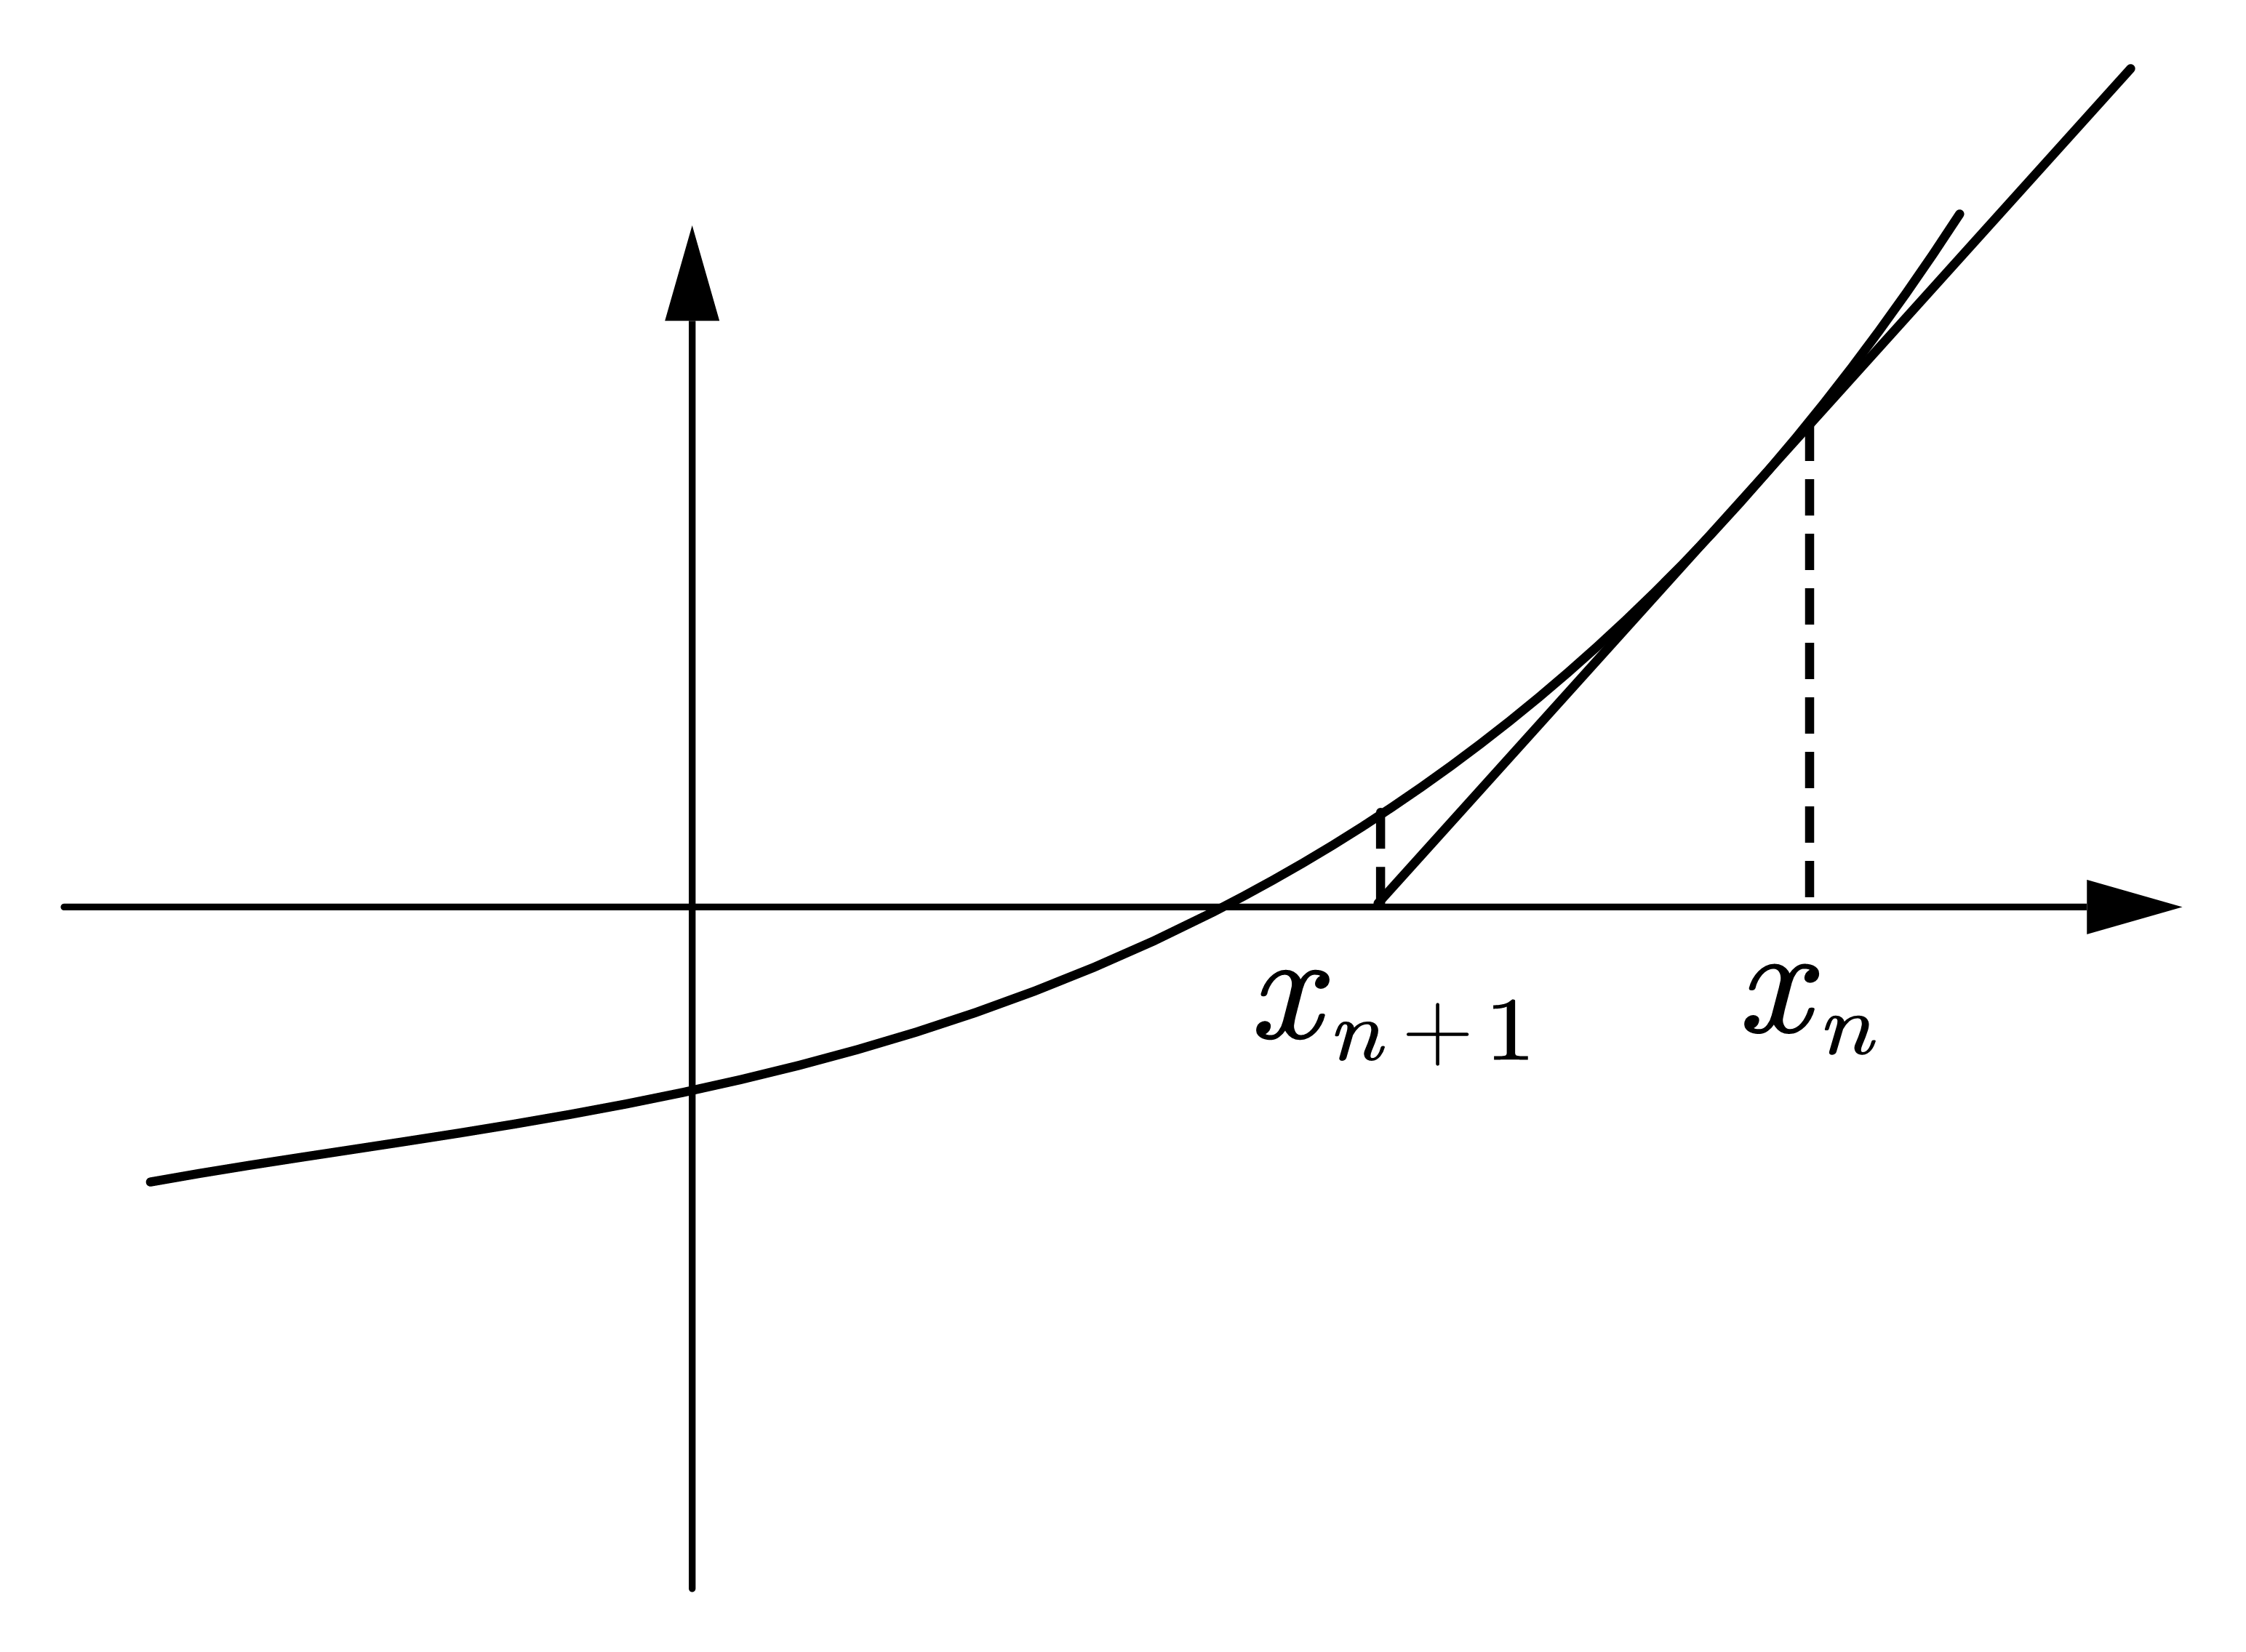
\includegraphics[width=8cm]{figure/Newton1D.png}
\end{center}

迭代过程为:
$$x_{n+1}=x_n-\frac{f(x_n)}{f'(x_n)}$$


\subsubsection{Secant方法}
牛顿迭代法中需要计算梯度,如果对梯度进行近似,可以得到其它一些方法.

$$f'(x_n)\simeq \frac{f(x_n)-f(x_{n-1})}{x_n-x_{n-1}}$$

迭代方法为
$$x_{n+1}=x_n-\frac{f(x_n)(x_n-x_{n-1})}{f(x_n)-f(x_{n-1})}$$

需要2个初始点,可以任选,或者计算一次导数,后面就不再需要计算导数了.

\subsection{解多元方程组}
求矩阵逆、伪逆也可以视为求多元方程组。
\subsubsection{不动点迭代}
\paragraph*{原始方法}对于方程
$$\bx=\bm{g}(\bx),\quad \bm{g}:\Rns\rightarrow \Rns$$
原始方法就是取$\bx_0$反复迭代到收敛。一个例子是
\begin{empheq}{align*}
x_1&=\frac{2\cos(x_2x_3)+1}{6}\\
x_2&=\frac{\sqrt{x_2^2+\sin x_3+1}}{9}-\frac{\sqrt{3}}{18}\\
x_3&=-\frac{e^{-x_1x_2}}{20}-\frac{10\pi-3}{60}
\end{empheq}
精确解为$\left[\inv{2},0,-\frac{\pi}{6}\right]$。
\paragraph*{Andreson加速}\label{andreson-fixed-point}新值是旧值的加权平均,权重通过优化残差得到。

取$\bm{f}_k=\bm{g}(\bx_k)-\bx_k$为残差。再取一个整数$m$作为分量数。算法:
\begin{enumerate}
\item 初始化$\bx_0,\bx_1=G(\bx_0),F_0$,
\item 对于$k\geq 1$,取$m_k=\min\{m,k\}$,装配矩阵$F=[\bm{f}_{k-m_k},\cdots,\bm{f}_k]$,就是取旧的$m_k$个值。求解最小二乘问题:
\begin{empheq}{align*}
\min_{\balpha}\quad & \|F\balpha\|_2\\
\text{s.t.}\quad & \balpha^T\bm{1}=1
\end{empheq}
根据拉格日乘数法,有
$$2F^TF\balpha=\lambda \bm{1}$$
则有
$$\balpha=\frac{\lambda}{2}(F^TF)^{-1}\bm{1}$$
代入$\balpha^T\bm{1}=1$可解出$\lambda$,然后有
$$\balpha=\inv{\bm{1}^T(F^TF)^{-1}\bm{1}}(F^TF)^{-1}\bm{1}$$

装配矩阵$G=[\bm{g}(\bx_{k-m_k}),\cdots, \bm{g}(\bx_k)]$,则新值为
$$\bx_{k+1}=G\balpha$$

在实现时,其实每一次不需要重新组装矩阵,只要$F,G$的列是对应的即可,因此可以这样,每一新分量加入到之前的下一列,如果装满了就填到第1列,然后第2列,……。

不过迭代几次后$f_k$就会趋于0,此时$F^TF$可能为奇异阵,因此不太可靠。需要使用更稳定的算法,参考\ref{linear-min-squared-prob}。
\end{enumerate}

以二分量为例,编程可以这样:
\begin{algorithm}
\SetKwData{Left}{left}\SetKwData{This}{this}\SetKwData{Up}{up}

\KwIn{$\bx_0$}
\KwOut{$\bx_k$}
\BlankLine
Initialization:\\
\quad$\bx_1=g(\bx_0)$\\
\quad$G=[\bx_1,g(\bx_1)]$\\
\quad$F=[g(\bx_0)-\bx_0,g(\bx_1)-\bx_1]$
\BlankLine
\For{$k=2$ \KwTo $n$}{
	求解$\balpha$\\
    $i=k \mod 2$\\
    $\bx_k=G\balpha$\\
	$G[,i]=g(\bx_k)$\\
	$F[,i]=g(\bx_k)-\bx_k$\\
}
\caption{2分量Anderson不动点迭代加速}
\end{algorithm}
从实践中来看,用Anderson加速可能初期很快,但由于浮点误差,可能最终得到的误差不如直接不动点。比如某个值的精确解为0,用不动点迭代6次到达$10^{-6}$,15次到达$10^L{-17}$,用Andreson加速,可能$3$次到达$10^{-6}$,但15次后可能只到$10^{-12}$。
\paragraph*{与梯度下降的关系}从某种意义上说,梯度下降法\ref{grade_descent}也是一种不动点迭代。

我们希望求解
$$g(\btheta)=\nabla f(\btheta)=0$$
则
$$J(g(\btheta))=\nabla^2 f(\btheta)$$
而且希望在这一点处是局部极小值。

取不动点迭代
$$\btheta=\btheta-\eta g(\btheta)$$
只要步长$\eta$取得足够小,则可以确保$\|\eta J\|\leq 1$,从而可以保证收敛性。

不动点迭代中取负梯度就是为了满足局部极小值,沿着负梯度方向,函数值下降,对应局部极小值。
\subsubsection{多元牛顿法}
直接把导数换成$J$矩阵:
$$\bx_{n+1}=\bx_n-\left(J(f(\bx_n)\right)^{-1}\bx_{n}$$

\subsubsection{Chebshev方法}
在\cite{li_chebyshev-type_2011}中对这种方法有比较详细的说明,该文章还推导了求伪逆的迭代方法。

\section{无约束多元函数优化}
以下默认是最小化.而且都需要提供初始值.

\subsection{梯度下降法系列}\label{gradient-descent-series}
只需要梯度信息。
\subsubsection{原始方法}\label{grade_descent}
无约束算法.属于一种最基本的算法,其它许多算法是根据这个算法改进而来.迭代过程为
$$\bx_{n+1}=\bx_n-\gamma \Delta F(\bx)$$

$\gamma$为步长,通常需要进行一维搜索得到,可以利用前面求解一元方程组的办法.

梯度下降法的变体主要集中在如何计算梯度以及选择的步长上面,有时还需要进行一些校正.

梯度下降法的一个有趣现象是,某点处的梯度要么与起始点的梯度平行,或者正交,这与等值面的法向量就是函数的梯度有关,也就是说,下降方向是等值面的法向量。而且下一个最优点就是等值面法线(1维)与另一个等值面的切点。如下图所示:

\begin{center}
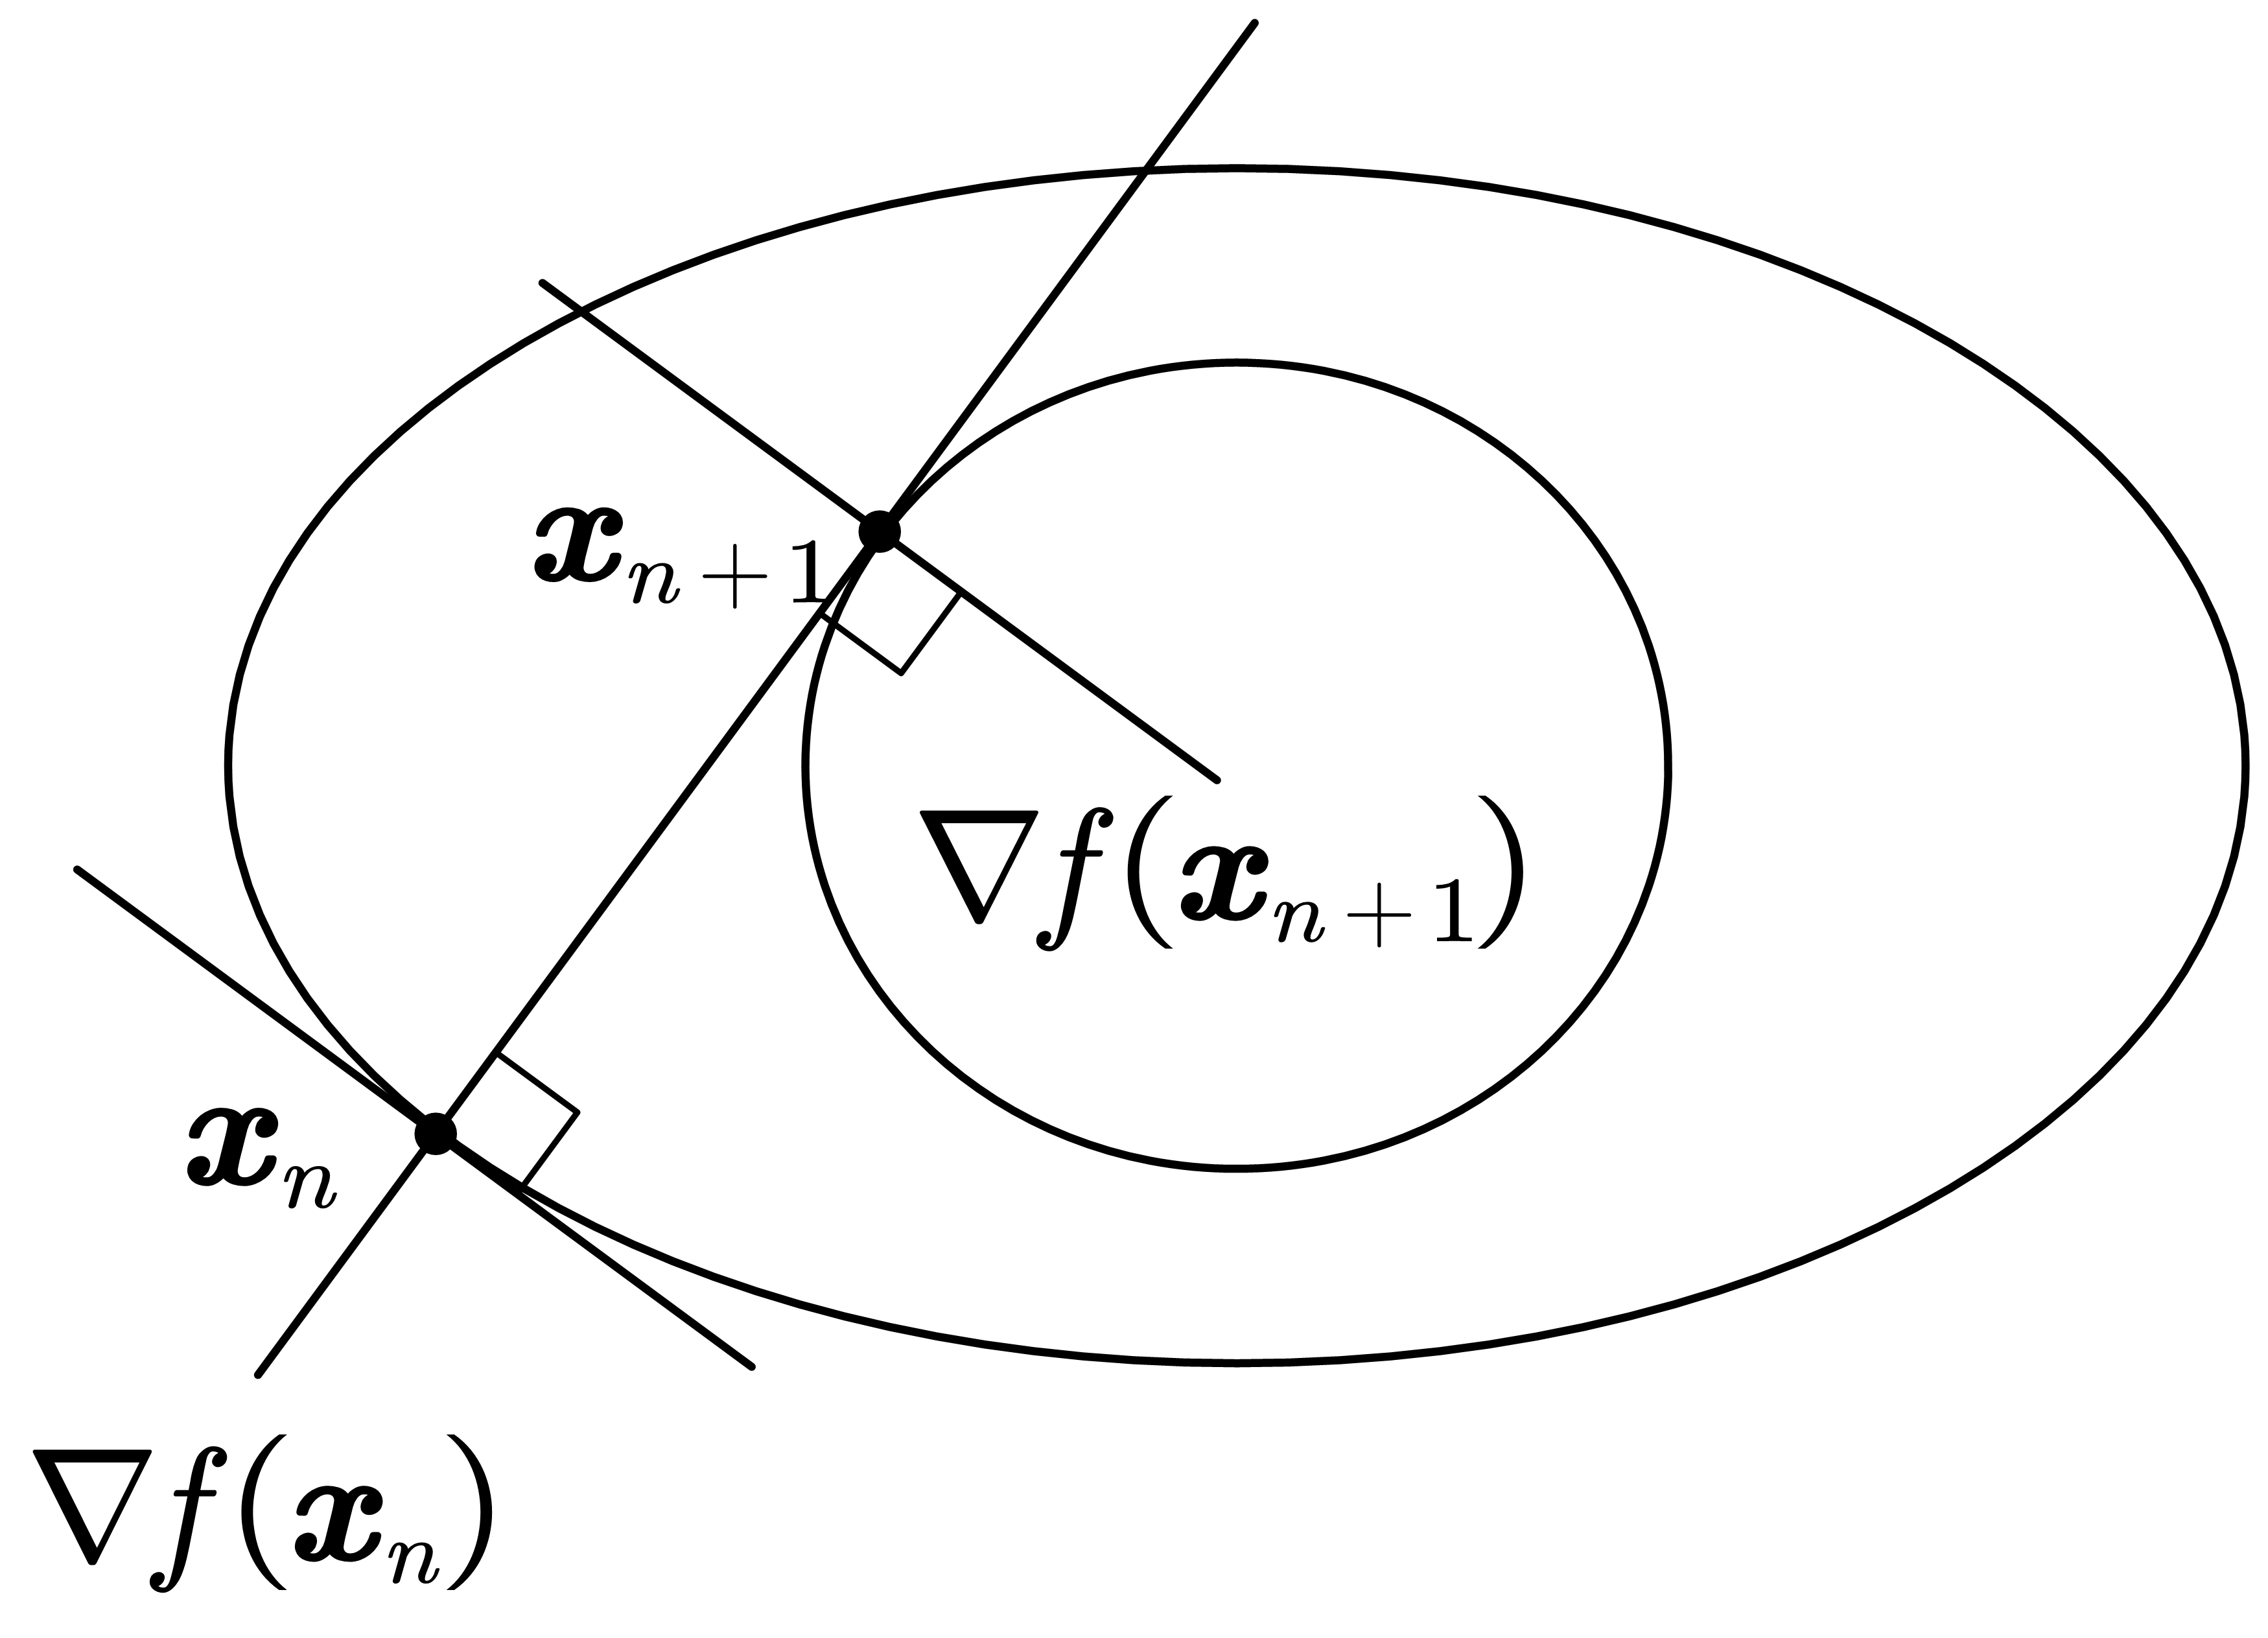
\includegraphics[width=6cm]{figure/grad_descent.png}
\end{center}

这一点也可以从迭代过程看出来,假如起始点为$\bm{x}^0$,现在进行梯度下降,则一维搜索的最优条件为
$$\pdv{f(\bx^0+\lambda \nabla f(\bx^0))}{\lambda}=\nabla f(\bx^0+\lambda \nabla f(\bx^0)))^T\nabla f(\bx^0)=\nabla f(\bx^1)^T\nabla f(\bx^0)=0$$
注意到第一次的下降方向是$\nabla f(\bx^0)$,第二次的下降方向是$\nabla f(\bx^1)$,两者内积为0,因此正交。
\subsubsection{随机梯度下降法}
对于机器学习,如果进行优化,就要计算全样本的梯度,如果每次只取一小部分甚至只取1个样本来计算,就是随机梯度下降.没有添加新的东西.不过步长现在不能再进行搜索了,只能固定,或者定期减小来稳定化.

\subsubsection{Adam}
\begin{empheq}{align*}
\bm{g}_{n}&=\nabla f(\bx_{n})	\\
\bm{m}_{n+1}&=\beta_1 \bm{m}_{n}+(1-\beta_1) \bm{g}_{n}\\
\bm{v}_{n+1}&=\beta_1 \bm{v}_{n}+(1-\beta_1) \bm{g}_{n}^2\\
\hat{\bm{m}}_{n+1}&=\frac{\bm{m}_{n}}{1-\beta_1^n}\\
\hat{\bm{v}}_{n+1}&=\frac{\bm{v}_{n}}{1-\beta_2^n}\\
\bx_{n+1}&=\bx_{n}-\frac{\alpha \hat{\bm{m}}_{n+1}}{\sqrt{\hat{\bm{v}}_{n+1}}+\varepsilon}
\end{empheq}

$\beta_1,\beta_2,\varepsilon$是预先确定的参数.通常$\beta_1,\beta_2$需要非常接近1,否则求指数后很快变成0了.原版论文的参数中,取$\beta_1=0.9,\beta_2=0.999,\varepsilon=10^{-8}$。$\alpha$就是学习率。$\bm{m}_0,\bm{v}_0$需要作为初始值给定,它们又被称为动量.注意到$\bm{m}_{n+1}$在$\beta_1=0.9$时,其中只有$1-0.9=0.1$倍直接计算的梯度,还是比较小的。

在实现时,只需要存储$\bm{m},\bm{v}$,可以通过就地修改来减少内存占用。但要看清楚,$\bm{m,v}$是自回归,不是对$\hat{\bm{m}},\hat{\bm{v}}$。另外需要注意的是迭代过程都是Elementwise计算。$n$的起始值不能为0,可以设成1。

在\cite{loshchilov2019decoupled}中提出了一种正则化方法,就是pytorch使用的\texttt{weight\_decay}。其公式是:
\begin{empheq}{align*}
\bm{g}_{n}'&=\bm{g}_n+\boxed{\lambda \bx_{n}}	\\
\bx_{n+1}'&=\bx_{n+1}-\boxed{\eta_t\lambda\bx_{n}}
\end{empheq}
$\lambda$对应decay,一般是取非常小的值。
\subsection{牛顿法系列}
\subsubsection{原始牛顿法}
\begin{empheq}{equation}
\bx^{(k+1)}=\bx^{(k)}-\nabla^2f(\bx^{(k)})^{-1}\nabla f(\bx^{(k)})
\end{empheq}
\subsubsection{拟牛顿法}
原始牛顿法需要计算$\nabla^2$的逆矩阵,这个非常难算,所以可以设法逼近它。记
\begin{empheq}{align*}
H_k&=\nabla^2f(\bx^{(k)})^{-1}\\
\bm{p}^{(k)}&=\bx^{(k+1)}-\bx^{(k)}\\
\bm{q}^{(k)}&=\nabla f(\bx^{(k+1)})-\nabla f(\bx^{(k)})
\end{empheq}

把$\nabla f(\bx^{(k)})$在$\bx^{(k+1)}$处展开后可以得到:
$$\nabla f(\bx^{(k)})=\nabla f(\bx^{(k+1)})+\nabla^2 f(\bx^{(k+1)})(\bx^{(k)}-\bx^{(k+1)})$$
变形即有
\begin{equation}
\bm{p}^{(k)}=H_{k+1}\bm{q}^{(k)}	\mtag{拟牛顿条件}
\end{equation}
取
$$H_{k+1}=H_{k}+\Delta H_{k}$$
可以用不同的方法来逼近这个$\Delta H_{k+1}$,这个矩阵也称为校正矩阵。

以下说明完整的过程:
\begin{enumerate}
\item 给定$\bx^{(0)}$计算一个初始的$H_0$,最优化$f(\bx^{(0)}-\lambda_0 H_0\nabla f(\bx^{(0)}))$得到$\lambda, x^{(1)}$.
\item 求$H_1,\bm{d}^{(1)},\lambda_1,\bx^{(2)}$。
\item 不断迭代上一步,直到停止。
\end{enumerate}

\paragraph*{秩1校正}假设矩阵的Rank是1,那么
$$\Delta H_k=\alpha_k \bz^{(k)}(\bz^{(k)})^T$$
$\alpha_k$是缩放系数。于是
\begin{empheq}{equation}\label{p-newton-rank-1}
\bm{p}^{(k)}=H_k\bm{q}^{(k)}+\alpha_k  \bz^{(k)}(\bz^{(k)})^T\bm{q}^{(k)}
\end{empheq}
这里表面上看未知数是$\alpha_k,\bz^{(k)}$,有$n+1$个,但方程是$n$个。实际上,$\alpha_k=\sign(\alpha_k)\sqrt{|\alpha_k|}^2$,所以它可以归约为$\pm 1$,因此只有$n+\inv{2}>n$个未知数,所以这个方程组是不定的,可能有多个解,即多种校正方法。

根据式\eqref{p-newton-rank-1}有
$$\bz^{(k)}=\frac{\bm{p}^{(k)}-H_k\bm{q}^{(k)}}{\alpha_k\bz^{(k)T}\bm{q}^{(k)}}$$
转置一下有:
$$\bz^{(k)}=\frac{(\bm{p}^{(k)}-H_k\bm{q}^{(k)})^T}{\alpha_k\bz^{(k)T}\bm{q}^{(k)}}$$
上两式相乘有
\begin{empheq}{equation}\label{p-newton-zzk}
\bz^{(k)}\bz^{(k)T}=\frac{(\bm{p}^{(k)}-H_k\bm{q}^{(k)})(\bm{p}^{(k)}-H_k\bm{q}^{(k)})^T}{\alpha_k^2(\bz^{(k)T}\bm{q}^{(k)})^2}
\end{empheq}

同时式\eqref{p-newton-rank-1}两边左乘$\bm{q}^{(k)T}$有
$$\bm{q}^{(k)T}(\bm{p}^{(k)}-H_k\bm{q}^{(k)})=\alpha_k(\bz^{(k)T}\bm{q}^{(k)})^2$$

这里给出了式\eqref{p-newton-zzk}的分子。所以
$$\Delta H_k=\frac{(\bm{p}^{(k)}-H_k\bm{q}^{(k)})(\bm{p}^{(k)}-H_k\bm{q}^{(k)})^T}{\bm{q}^{(k)T}(\bm{p}^{(k)}-H_k\bm{q}^{(k)})}$$

\paragraph*{DFP方法}公式如下:
\begin{empheq}{equation}\label{p-newton-DFP}
\Delta H_k=\frac{\bm{p}^{(k)}\bm{p}^{(k)T}}{\bm{p}^{(k)T}\bm{q}^{(k)}}-\frac{H_k\bm{q}^{(k)}\bm{q}^{(k)T}}{\bm{q}^{(k)}H_k\bm{q}^{(k)T}}
\end{empheq}

\paragraph*{BFGS}公式如下
\begin{empheq}{align}\label{p-newton-BFGS}
\Delta H_k&=\left(1+\frac{\bm{q}^{(k)T}H_k\bm{q}^{(k)}}{\beta}\right)\frac{\bm{p}^{(k)}\bm{p}^{(k)T}}{\beta}-\frac{\bm{p}^{(k)}\bm{q}^{(k)T}H_k+H_k\bm{q}^{(k)}\bm{p}^{(k)T}}{\beta}\\
\beta_k&=\bm{p}^{(k)T}\bm{q}^{(k)}
\end{empheq}

取
$$\bm{q}^{(k)}=B_{k+1}\bm{p}^{(k)}$$
然后利用DFP方法\eqref{p-newton-DFP}可以得到$B_{k}$的递推公式,再求逆:
$$H_{k+1}=B_{k+1}^{-1}$$
即可得到BFGS方法\eqref{p-newton-BFGS}。
\subsection{共轭梯度法}
\subsubsection{概念}
\begin{definition}[共轭梯度]\label{conjugate-gradient}
$A$为正定矩阵,如果$\bm{d}^{(1)},\bm{d}^{(2)}\in\mathbb{R}^n$满足
$$\bm{d}^{(1)T}A\bm{d}^{(2)}=0$$
称$\bm{d}^{(1)},\bm{d}^{(2)}$关于$A$共轭(正交)。
\end{definition}
%取Cholesky分解$A=LL^{T}$
以下给出一些关于共轭梯度有关的例子:
\begin{example}
$A$为一正定矩阵,$\bm{p}^{(i)},i\in\{1,\cdots,n\}$关于$A$共轭,给定某$\bx\in\mathbb{R}^n$,试求$\bx$在基$\bm{p}^{(i)}$下的坐标。
\end{example}
\begin{solution}
假设$\bx=\sum \alpha_i \bm{p}^{(i)}$,则
$$\bm{p}^{(i)}A\bx=\alpha_i\bm{p}^{(i)}A\bm{p}^{(i)}$$
于是
$$\alpha_i=\frac{\bm{p}^{(i)}A\bx}{\bm{p}^{(i)}A\bm{p}^{(i)}}$$
\end{solution}
\subsubsection{计算过程}
基本原理是每隔$n$次用最速下降方向“重启”,否则用其它方法对搜索方向校正。

计算步骤如下:
\begin{enumerate}
\item 给定初始点$\bx^{(1)}$,取$\by^{(1)}=\bx^{(1)},\bm{d}^{(1)}=-\nabla f(\by^{(1)}),k=j=1$。
\item\label{conjudate-gradient-1d-search} 假如$\|\nabla f(\by^{(1)})\|\leq \varepsilon$,停止。否则进行一维搜索,求解
$$\min_{\lambda \geq 0}f(\by^{(j)}+\lambda_j \bm{d}^{(j)})$$
得到$\by^{(j+1)}$。
\item 如果$j<n$, 进行步骤\ref{conjudate-gradient-calibrate};否则,进行步骤\ref{conjudate-gradient-restart}(重置)。
\item\label{conjudate-gradient-calibrate}  校正方向。取$\bm{d}^{(j+1)}=-\nabla f(\by^{(j+1)})+\beta_j \bm{d}^{(j)}$,其中
$$\beta_j=\frac{\|\nabla f(\bm{y}^{(j+1)})\|^2}{\|\nabla f(\bm{y}^{(j)})\|^2}$$
取$j\coloneqq j+1$。
\item\label{conjudate-gradient-restart}取$\bx^{(k+1)}=\by^{(n+1)},\by^{(1)}=\bx^{(k+1)},\bm{d}^{(1)}=-\nabla f(\by^{(1)}),j=1,k\coloneqq k+1$,转步骤\ref{conjudate-gradient-1d-search}。
\end{enumerate}
$k$是全局迭代次数。
\subsection{信赖域法}

\subsection{各种方法的比较}

\section{约束多元函数优化}
\subsection{最小二乘}
\subsubsection{线性约束最小二乘}\label{linear-min-squared-prob}
在不动点迭代的Andreson方法\ref{andreson-fixed-point}中需要求解以下问题:
\begin{empheq}{align*}
\min_{\balpha}\quad & \|F\balpha\|_2,F\in\mathbb{R}^{n\times k}\\
\text{s.t.}\quad & \balpha^T\bm{1}=1
\end{empheq}
如果直接求解的话,由于$F^TF$通常条件数很大,不能求逆,需要更稳定的方法。以下说明一种基于零空间的方法:
\paragraph*{Null-space方法},首先取$\bm{v}=[0,0,\cdots,1]^T\in\mathbb{R}^{k}$,假设存在满秩矩阵$V\in\mathbb{R}^{k\times (k-1)}$满足$\bm{1}^TV=\bm{0}$,则可以令$\balpha=\bm{v}+V\bm{\gamma}$,原问题转换为一个无约束优化问题:
\begin{empheq}{align*}
\min_{\bm{\gamma}}\quad & \|F(\bm{v}+V\bm{\gamma})\balpha\|_2=\bm{d}_k+FV\bm{\gamma}
\end{empheq}
$\bm{d}_k$就是$F$的最后一列。一阶条件为
$$(DV)^TDV\bm{\gamma}=-(DV)^TD\bm{\gamma}$$
$(DV)^T$条件数也还是很大,可以使用QR分解,取$DV=QR$,则一阶条件变成
$$R\bm{\gamma}=-Q^T\bm{d}_k$$
求解上式即可。最后$\bm{\alpha}=\bm{v}+V\bm{\gamma}$。
\subsection{可行方向法}
\subsubsection{Zoutendijk法}
\paragraph*{线性约束}求解线性等式、不等式约束问题\ref{constrained-lin-eq-neq}的Zoutendijk方法如下:
\begin{enumerate}
\item 给定初始点$\bx^{(1)}$,取$k=1$。
\item\label{zoutendijk-linear-2}把不等式约束条件分解为起作用与不起作用约束:
\begin{empheq}{equation}
A=\begin{bmatrix}
A_1\\A_2
\end{bmatrix},\bm{b}=\begin{bmatrix}
\bm{b}_1\\\bm{b}_2
\end{bmatrix}
\end{empheq}
其中$A_1\bm{x}^{(k)}=\bm{b}_1,A_2\bm{x}^{(k)}\geq \bm{b}_2$。需要强调的是,$\bx\geq \bm{0}$也属于约束条件,不要忘记。计算$\nabla f(\bx^{(k)})$。
\item 求解线性规划:
\begin{empheq}{equation}
\begin{aligned}
&\min && \nabla f(\bx^{(k)})^T\bm{d}\\
	&\text{s.t. } && A_1\bm{d}\geq \bm{0}\\
	& && E\bm{d}=\bm{0}\\
	& && -1\leq \bm{d}\leq 1
\end{aligned}
\end{empheq}
得到最优解$\bm{d}^{(k)}$。
\item 如果$\nabla f(\bx^{(k)})^T\bm{d}^{(k)}=0$。停止计算,得到K-T点。否则进行下一步。
\item\label{zoutendijk-lin-1d-search} 一维搜索。首先计算范围。取
\begin{empheq}{align}
\hat{\bm{b}}&=\bm{b}_2-A_2\bx^{(k)}\\
\hat{\bm{d}}&=A_2\bm{d}^{(k)}
\end{empheq}
然后令
\begin{empheq}{equation}
\lambda_{\max}=\begin{cases}
\min\  \left\{\frac{\hat{b}_i}{\hat{d}_i}\rvert \hat{d}_i<0\right\}& \hat{\bm{d}}\ngeq \bm{0}\\
\infty & \hat{\bm{d}}\geq \bm{0}
\end{cases}
\end{empheq}
$\hat{\bm{b}}$实际上是不起作用约束条件的“残差”,限定了调整范围。

进行一维搜索
\begin{empheq}{equation}
\min_{\lambda\in [0,\lambda_{\max}]} f(\bm{x}^{(k)}+\lambda \bm{d}^{(k)})
\end{empheq}
得到最优解$\lambda_k$,同时计算$\bx^{(k+1)}$。这里在计算时不要忘记$\lambda_{\max}$。
\item 取$k\coloneqq k+1$,返回\ref{zoutendijk-linear-2}。
\end{enumerate}


\subsubsection{梯度投影法系列}
\paragraph*{基本梯度投影法}
属于最速下降法的推广。求解线性等式、不等式约束问题\ref{constrained-lin-eq-neq}的基本梯度投影方法如下:
\begin{enumerate}
 \item 给定初始点$\bx^{(1)}$,取$k=1$。
\item\label{gradient-project-linear-2}把不等式约束条件分解为起作用与不起作用约束:
\begin{empheq}{equation}
	A=\begin{bmatrix}
		A_1\\A_2
	\end{bmatrix},\bm{b}=\begin{bmatrix}
		\bm{b}_1\\\bm{b}_2
	\end{bmatrix}
\end{empheq}
其中$A_1\bm{x}^{(k)}=\bm{b}_1,A_2\bm{x}^{(k)}\geq \bm{b}_2$。
\item\label{gradient-project-linear-3} 令
\begin{empheq}{align*}
M&=\begin{bmatrix}
A_1\\E
\end{bmatrix}\\
P&=\begin{cases}
I & M\in \emptyset\\
I-M^T(MM^T)^{-1}M & \text{否则}
\end{cases}
\end{empheq}
\item 计算下降方法。令$\bm{d}^{(k)}=-P\nabla f(\bx^{(k)})$。如果$\bm{d}^{(k)}\neq \bm{0}$,转步骤\ref{gradient-project-linear-6};如果$\bm{d}^{(k)}=0$,转步骤\ref{gradient-project-linear-5}。
\item\label{gradient-project-linear-5} 如果$M$空,则停止计算。否则令
$$W=(MM^T)^{-1}M\nabla f(\bx^{(k)})=\begin{bmatrix}
	\bm{u}\\\bm{v}
\end{bmatrix}$$
如果$\bm{u}\geq \bm{0}$,停止计算。如果包含负分量,取一个负分量$u_j$,去掉$A_1$中$u_j$对应的行,返回步骤\ref{gradient-project-linear-3}。
\item\label{gradient-project-linear-6} 一维搜索。这一步与Zoutendijk法中步骤\ref{zoutendijk-lin-1d-search}相同。
\item 取$k\coloneqq k+1$,返回\ref{gradient-project-linear-2}。
\end{enumerate}
\paragraph*{Frank-Wolfe方法}属于梯度投影法的一个变种。求解线性等式约束问题\ref{constrained-lin-eq}的Frank-Wolfe方法如下。

以下记$S=\{\bx|A\bx=\bm{b},\bx\geq \bm{0}\}$,即线性约束的可行域。

\begin{enumerate}
 \item 给定初始点$\bx^{(1)}$,取$k=1$。
 \item\label{frank-wolfe-lin-linear} 求解线性规划:
 \begin{empheq}{equation}
 \min_{\bx\in S} \nabla f(\bx^{(k)})^T\bx
 \end{empheq}
得到最优解$\by^{(k)}$。
\item 如果$\nabla f(\bx^{(k)})^T(\by^{(k)}-\bx^{(k)})\leq \varepsilon$,停止计算。否则进行下一步。
\item\label{frank-wolfe-lin-1d} 从$\bx^{(k)}$出发,沿方向$\by^{(k)}-\bx^{(k)}$在线段$\by^{(k)},\bx^{(k)}$上进行一维搜索:
\begin{empheq}{equation}
\min_{\lambda in [0,1]} f(\bx^{(k)}+\lambda (\by^{(k)}-\bx^{(k)}))
\end{empheq}
得到$\lambda_k$。
\item 更新
$$\bx^{(k+1)}=\bx^{(k+1)}+\lambda_k (\by^{(k)}-\bx^{(k)})$$返回步骤\ref{frank-wolfe-lin-linear}。
\end{enumerate}
注意在以上步骤\ref{frank-wolfe-lin-1d}进行一维搜索时,不需要计算上界,上界是已知的,即1。

\subsection{罚函数法}
\subsubsection{基本原理}
罚函数法在Matlab的\texttt{solve}中有应用(Interior Point算法)。实质是把约束条件整合进目标函数。于是可以当成一个无约束问题来做,跟多目标优化很像。分为外点与内点罚函数法。前者的搜索空间是在可行域外部,不断靠近可行域;而后者的搜索空间是在可行域内部。对于等式约束,可行域内部是"空的",所以此时不能用原始的内点法。

限定搜索空间在内部是通过障碍函数$G(\bx,r)$实现的,比如在内点法中,定义为
$$G(\bx,r)=f(\bx)+rB(\bx)$$
当$\bx$趋于边界(具体地是$g_i(\bx)\rightarrow 0^+$,一般要求约束条件形如$\bm{g}(\bx)\geq \bm{0}$)时,$B(\bx)\rightarrow +\infty$。常见的两种函数为
\begin{empheq}{align*}
B(\bx)&=\sum_{i=1}^{m}\inv{g_i(\bx)}\\
B(\bx)&=-\sum_{i=1}^{m}\log g_i(\bx)
\end{empheq}
令$r\rightarrow 0$,相当于极小化$f$,同时由于$B$函数的趋于无穷大的限制,使得解尽可能靠近边界,从而趋近于最优解。

外点法是类似的,其目标函数是
\begin{empheq}{align*}
F(\bx,\sigma)&=f(\bx)+rP(\bx)\\
P(\bx)&=\sum_{i=1}^{m}\phi(g_i(\bx))+\sum_{i=1}^{n}\varphi(h_i(\bx))
\end{empheq}
$\sigma$为罚因子,通常要取得大一些。$\phi$和$\varphi$通常取为
\begin{empheq}{align*}
\phi&=\left[\max\{0,-g_i(\bx)\}\right]^{\alpha}\\
\varphi&=\|h_i(\bx)\|^\beta
\end{empheq}
一般来说$\alpha=\beta=2$,就是2-范数。而且可以看出$\phi$里面是$\ReLU$函数。外点法的含义是很明显的,就是解在可行域内部时没有惩罚,在外部时有很大的惩罚。

令$r\rightarrow \infty$,可以得到解析解。
\subsubsection{外点罚函数法}
\begin{example}
\begin{empheq}{equation}
\begin{aligned}
\min\ & (x_1-3)^2+(x_2-2)^2\\
\text{s.t. } & x_1+x_2=4
\end{aligned}
\end{empheq}
\end{example}

\begin{solution}
取目标函数
$$f(x_1,x_2)=(x_1-3)^2+(x_2-2)^2+\sigma(x_1+x_2-4)^2$$
根据一阶条件,解一个线性方程组得到:
$$\bx=\frac{1}{2\sigma+1}\begin{bmatrix}
5\sigma+3\\3\sigma+2
\end{bmatrix}$$
令$\sigma\rightarrow \infty $,有
$$\bx=\begin{bmatrix}
\frac{5}{2}\\\frac{3}{2}
\end{bmatrix}$$
\end{solution}

\subsubsection{内点罚函数法}
\begin{example}
	\begin{empheq}{equation}
		\begin{aligned}
			\min\ & \inv{12}(x_1+1)^3+x_2\\
			\text{s.t. } & x_1\geq 1,x_2\geq 0
		\end{aligned}
	\end{empheq}
\end{example}

\begin{solution}
取目标函数:
$$G(\bx,r)=\inv{12}(x_1+1)^3+x_2+r\left(\inv{x_1-1}+\inv{x_2}\right)$$

由一阶最优性条件有:
$$\bx=\begin{bmatrix}
\sqrt{1+2\sqrt{r}}\\
\sqrt{r}
\end{bmatrix}$$
令$r\rightarrow 0$,有
$$\bx=\begin{bmatrix}
	\sqrt{1}\\
	\sqrt{0}
\end{bmatrix}$$
\end{solution}